\section{Grundlagen}
\label{sec:Grundlagen}
In diesem Kapitel werden die theoretischen Grundlagen, welche zum Verständnis der vorliegende Arbeit wichtig sind, beschrieben. Zu Beginn erfolgt ein kurzer Einstieg in die Optimierungsgrundlagen. Dann folgt die Einführung in die Grundlagen der Genetischen Algorithmen. Anschließend werden die wichtigen Grundlagen der Künstlichen Neuronalen Netzen erklärt. Zum Schluss wird kurz auf die Hyperparameter und ihre Besonderheiten eingegangen.

\subsection{Optimierungsgrundlagen}
Angenommen es soll ein Künstliches Neuronales Netz mit k Layern und L Neuronen zur Klassifizierung von einfachen handgeschriebenen Zahlen erstellt werden. Der Entwickler entscheidet sich für ein 3 Layern Netz mit jeweils 3 Neuronen. Nach dem Training hat es die Genauigkeit von 85 Prozent. Nun kann man nicht sicher sagen, ob für k = 3 und l = 3  die optimale Lösung gefunden wurde. Um dies beurteilen zu können, müssen viele Experimente durchgeführt werden. Die Frage ist, wie kann man die besten Werte für k und j finden, um die Klassifizierung zu maximieren? Dieser Vorgang, speziell im Zusammenhang mit Künstlichen Neuronalen Netzen, wird als Hyperparameter-Optimierung bezeichnet. Bei der Optimierung wird mit einem Initialwert gestartet, dieser ist in den seltensten Fällen die exakte Lösung. Dieser Initialwert muss einige Male verändert werden, um auf ein Optimum zu kommen. Manchmal ist dieses Optimieren so komplex, dass es durch eine Funktion ersetzt werden muss. In diese Arbeit ist dafür der Genetische Algorithmus zuständig.

Ractical Computer Cision Apllica ss.130

\subsection{Genetische Algorithmen}

Die Inhalte des folgenden Abschnittes sind, sofern nicht anderweitig angeführt, aus den Grundlagenbüchern xxxx und xxxx übernommen. 
Genetische Algorithmen sind heuristische Suchansätze. Im Wesentlichen zeichnet sie eine probabilistische Eltern Selektion als primären Suchoperator aus. Als weitern Suchoperator kann noch auf die Mutation zurückgegriffen werden. Dieser garantiert eine Erreichbarkeit aller Punkte im Suchraum und erhält die Grunddiversität in der Population. Es gibt zwei verschiedene Algorithmen der Standart-GA tauscht nach einer Generation die komplette Elternpopulation durch die Kinderpopulation aus. Und bestehen in der Regel immer aus fünf gleichen Schritten wie in Abb. \ref{fig:Ablauf_kurz} zusehen ist. Im Gegensatz dazu gibt es den Steady-State-GA, welcher durch seine überlappende Population auszeichnet, dieser Algorithmus wird in der Arbeit nicht verwendet und wird deswegen nicht weiter erklärt.

Evolutionäre Algo -- s.128 und Seite - 11 Genetic Algorithm Essentials

\noindent%
\begin{figure}[H]
  \centering  
  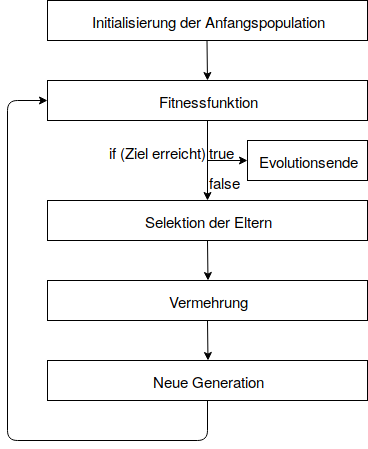
\includegraphics[scale=0.6]{img/Ablauf_kurz.png}
  \caption{Ablaufdiagramm eines Genetischen Algorithmuses mit 5 Schritten}
  \label{fig:Ablauf_kurz}
\end{figure}


Der Standard genetische Algorithmus \ref{GA} besteht aus folgenden 5 Schritte: \\
Schritt 1, Initialisieren der Anfangspopulation.	\\
Schritt 2, Fitness berechnen mit Hilfe der Fitnessfunktion.	\\
Schritt 3, Selektieren der Eltern.	\\
Schritt 4, Vermehren durch Crossover und Mutation.	\\
Schritt 5, Austausch der Populationen.	\\
In den nachfolgenden Unterkapiteln werden auf die einzelnen Schritte genauer eingegangen.	 \\

\begin{algorithm}
\caption{Basic Genetischer Algorithm }
\begin{algorithmic}[1]
\State Initialisieren der Anfangspopulation   \Comment{put some comments here}
\While{$ Fitness \leq Abbruchbedingung$}
	\State Fitness aller Individuen Berechnen
	\State Selektieren der Eltern
	\State Vermehren durch Cross-over und Mutation
	\State Austausch der Populationen
\EndWhile

\label{GA}
\end{algorithmic}
\end{algorithm}

Im folgenden Kapitel werden auf diese 5 Schritte des Genetischen Algorithmus \ref{GA} näher eingegangen. Zuerst wird auf Aufbau und die Initialisierung eingegangen. Anschließend folgt eine Zusammenfassung der Fitnessfunktion. Darauffolgend werden Verschiedene Möglichkeiten für die Eltern Selektion dargelegt. Anschließend wird die Vermehrung durch Crossover und Mutation erklärt. Zum Schluss wird noch auf den Austausch der Populationen eingegangen. 


\iffalse
Genetische Algorithmen sind im Wesentlichen durch eine probabilistische Eltern selektion und die Rekombination als primären Suchoperator gekennzeichnet.Die Mutation ist meist nur ein Hintergrundoperator, der mit einer geringen Wahrschenlichkeit zur anwendungkommt. Er garantiert die Erreichbarkeit aller Punkte im Suchraum und erhält eine Drunddiversitöt in der Population.

Evolutionäre Algo -- s.128


Genetische Algorithmen sind heuristische Suchansätzem, die auf einer breitenbasis von Optimierungsproblemen angewendet werden können. Diese Flexibiliät macht sie für die Praxis für viele sehr attraktiv.Die Evulution ist Grundlage des Genetischen Aglorithmuses. durch die aktuelle Vielfalt und der Erfolg der Arten ist dies schon alleine ein guter Grund sich diesen Optimierungs Algortihmus näher anzuschauen. Denn sdiese Arten sind in der lage sich an ihre Umgebung anzupassen und sich zu zu komplexen Strukturen zuentwickelen, und somit das überleben in verschiedesten Umgebungen eröglichen. Hierbei ist die Paarung und Entwicklung von Nachkommen eine der Hauptprinipen des Erfolges der Evolution. In diesem Kapitel werden wir die Grundlage der GEnetischen Algorithmen näher anzuschauen. Beginnen wir mit der grundlage das es sich bei den Genetischen Algorithmen um einen Polulations ansatz handelt. Anschließend wird auf die wichtigesten genetischen Operatioren vorstellen darunter gehöhren, Selektion, Crossover und Muttation

Seite - 11 Genetic Algorithm Essentials


Algorithmus 1 zeigt den Pseudocode des grundlegenden genetischen Algorithmus, der Folgendes kann dienen als Blaupause für viele verwandte Ansätze. Am Anfang eine Reihe von Lösungen,die als Population bezeichnet wird, wird initialisiert. Diese Initialisierung wird empfohlen.um zufällig den gesamten Lösungsraum abzudecken oder um Experten zu modellieren und einzubinden. Wissen. Die Darstellung bestimmt den Initialisierungsprozess. Für BitfolgeDarstellungen ist eine zufällige Kombination von Nullen und Einsen sinnvoll, z.B.das anfängliche Zufallschromosom 1001001001001 als typische Bitfolge der Länge 10. Der Hauptgenerationskreislauf des Genetischen Algorithmus erzeugt neue Nachkommen.Kandidatenlösungen mit Crossover und Mutation, bis die Bevölkerung vollständig ist.

Seite - 11 Genetic Algorithm Essentials
\fi 

\subsubsection{Aufbau und Initialisierung  der Population}
Der klassische genetische Algorithmus basiert auf einer Reihe von Kandidatenlösungen. Die Größe der Population ist somit auch die Anzahl der Lösungen. Jede Lösung kann als einzelnes Individuum gesehen werden und wird durch ein Chromosomenstrang repräsentiert. Ein Chromosom besteht wiederum aus vielen Genen, welche die Hyperparameter repräsentieren. Der Aufbau ist grafisch in Abbildung \ref{fig:population} dargestellt. Es gibt verschiedene Möglichkeiten, diese Gene dazustellen. Um die Grundlagen nahe des später folgenden Konzepts zuhalten, wird der Ablauf per Dezimal-Genen erklärt.



\noindent%
\begin{figure}[H]
  \centering  
  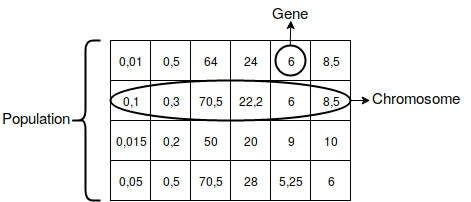
\includegraphics[scale=0.7]{img/population.png}
  \caption{Beispiel einer Population mit 4 Induviduen (Chromsomen) welche 6 dezimale Gene besitzen}
  \label{fig:population}
\end{figure}

Diese Anfangspopulation (Generation 0) wird zufällig initialisiert, um die größt mögliche Abdeckung des Suchraums zu gewähren. Die erste Generation besitzt eine sehr geringe Fitness, welche im verlauf des Trainings stetig steigert bis sie das Maximum erreicht. (XXXFachbegriffxx)


\subsubsection{Fitnessfunktion}
Die Fitnessfunktion (engl. Fitnessfunction) bewertet das Individuum anhand seiner Funktionstauglichkeit, bezogen auf die vorhandene Aufgabe. Dabei werden nicht einzelnen Gene bewertet, sondern das ganze Chromosom. Es gibt keine universelle Fitnessfunktion, diese muss also für jede Anwendung speziell geschrieben werden. Es wird nicht berücksichtigt welches Gene sich positiv bzw. negativ auswirken. Als Rückgabewert gibt die Fitnessfunktion uns einen dezimalen/float Fitnesswert. Dabei steht ein höherer Fitnesswert stehst für eine höher Qualität an Individuum sprich bessere Lösung.

Practical Computer Vison Apllica s.134


\subsubsection{Selektion der Eltern}
Bei dem Schritt Selektion (engl. Select Parents) geht es darum einen Elternpool zu generieren, aus welchem die neue Generation erstellt wird. Deshalb ist es wichtig, nur die Besten, geeignetesten Individuen auszuwählen. Es gibt verschiedene Ansätze bei der Selektion, die elementar wichtigsten werden genannt und erläutert.

Informationen wurden aus dem Paper \cite{shukla15} entnommen.


\begin{itemize}
\item \textbf{Auswahl proportional zur Fitness (engl. Fitness Proportonal Selction(FPS))} Die Eltern werden nach ihrer Fitness proportional ausgewählt und zum Elternpool hinzugefügt. Wenn $f(a_i)$ die Fitness des Individuell $a_i$ in der Population ist, dann ist die Wahrscheinlichkeit selektiert/ausgewählt zu werden:
\begin{equation}
	ps(a_i) = \frac{f(a_i)}{\sum_{i=1}^n f(a_j)}; j\in{1,2,...,n} \label{eq:1}
\end{equation}
wobei n die Anzahl der Individuen einer Population ist.
Diese Wahrscheinlichkeit $ps$ kann man sich als Anteil auf einem Rouletterad, wie in Abblidung \ref{fig:roulette_wheel} vorstellen. Auf dem zufällig die Eltern aus den Individuen $a1,..,an$ \glqq ausgedreht \grqq werden. Dieser Ansatz hat leider das Problem, dass Individuen die am Anfang sich als gut beweisen, schnell die ganze Population übernehmmen. Das kann dazuführen, dass eine mögliche bessere Lösung durch den Algorithmus im Suchraum nicht gefunden wird.

\begin{figure}[htb]
  \centering  
  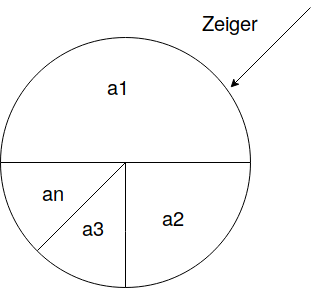
\includegraphics[scale=0.5]{img/roulette_wheel.png}
  \caption{Rouletterad mit proportinalen Anteil der Individuen anhand ihrere Fitness}
  \label{fig:roulette_wheel}
\end{figure}

introduction to evolutionary comp s80

\item \textbf{Ranking Selektion} Diese Selektion wurde von Backer als Verbesserung der Fitness Proportonal Selection entwickelt \cite{baker1985adaptive}. Dabei werden die Eltern nicht direkt nach ihrer Fitness ausgewählt. Die Fitness dient nur zum Einteilen in eine Rangliste. Anhand dieser Rangliste wird dann wieder mit Hilfe des Rouletterades ausgewählt. Dabei gibt es verschiedene Verfahren wie diese Verteilung aussehen kann:

Das lineare Ranking:
\begin{equation}	
	p_i = \frac{1}{N}(n^- + (n^+ - n^- ) \frac{i-1}{N-1}; i\in{1,...,N} \label{eq:2}
\end{equation}
Wobei $p_i$ die Wahrscheinlichkeit des Individuums ist selektiert zu werden. $\frac{n^-}{N}$ ist die Wahrscheinlichkeit des schlechtesten Individuums selektiert zu werden und  $\frac{n^+}{N}$ ist die Wahrscheinlichkeit des besten Individuums selektiert zu werden.

Das expontienelle Ranking:
\begin{equation}
	p_i = \frac{c^{N-i}}{\sum_{j=1}^N c^{N-j}}; i\in{1,...,N} \label{eq:3}
\end{equation}
die Summe $\sum_{j=1}^N c^{N-j}$ normalisiert die Wahrscheilichkeit um Sicherzustellen das $\sum_{i=1}^N p_i = 1$.
Wobei die Berechnungen \ref{eq:2} und \ref{eq:3} nur den Anteil eines Individuums auf dem Rouletterades verändern.

\item \textbf{Tunier Selektion} In diesem Verfahren werden zufällig k Induviduuen der Population ausgewählt. Diese k Individuen treten wie in einem Tunier gegeneinander an. Der Gewinner ist das Individuum mit dem besten Fitnesswert, dieser wird dann auch als Elternteil ausgewählt. Hierbei wird auf den Elternpool verzichtet und direkt ein Kind aus zwei Gewinnern erstellt. Eingesetzt wird dies bei kleineren Populationen mit weniger als 20 Individuen.

\begin{figure}[htb]
  \centering  
  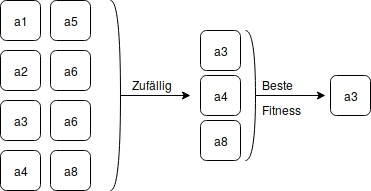
\includegraphics[scale=0.7]{img/tunier.png}
  \caption{Tunier Selektion mit k = 3 Individuen und dem Gewinner Individuum 3}
  \label{fig:roulette_wheel}
\end{figure}


\end{itemize}


\subsubsection{Vermehrung}
Aus dem Elternpool werden nun Nachkommen (neue Individuuen) geschaffen. Alleine durch die Paarung(engl. Crossover) von qualitativ hochwertigen Individuen wird erwartet, dass die Nachkommen eine bessere Qualität besitzen als die ihrer Eltern. Als zweite Verbesserung wird noch die Mutation einzelner Gene angewendet. Für Crossover und Mutation gibt es verschiedene Ansätze, die in diesem Abschnitt genauer erklärt werden.

\paragraph{Crossover} nennt man die Operation, bei der die Chromostränge der Kinder Individuen zusammengesetzt werden.
Beim Crossover gibt es mehrer Varianten, die Ein-Punkt-Crossover (engl. One-Point-Crossover), in welchem zufällig ein Punkt im Chromsomenstrang festgelegt wird.
Ab diesem Punkt wird der Chromosomenstrang dann aufgeteilt und anschließend mit dem Crossover des anderen Elternteils wieder zusammen gesetzt. Ein einfaches Beispiel ist im Oberenteil der Abbildung \ref{fig:chromoson_crossover} zu sehen.

Eine Abwandlung des Ein-Punkt-Crossover ist das Zwei-Punkt-Crossover oder k-Punkt-Crossover. Hier wird der Chromsomenstrang an k Punkten aufgeteilt und anschließend mit dem Anteil des zweiten Elternteil wieder zusammengesetzt.
In mittleren Teil der Abbildung \ref{fig:chromoson_crossover}
ist ein k = 2 Crossover oder auch zwei-punkt-crossover (engl. two-point-crossover) zu sehen.

Eine weitere grundlegende Operation beim Crossover ist die Uniform-crossover \cite{Syswerda1989} in welcher es keine festgelegte Anzahl an Punkten gibt. Hier wird für jedes Gen zufällig entschieden aus welchem Elternteil das Gen entnommen wird.
Dies im unteren Teil der Abbildung \ref{fig:chromoson_crossover} noch einmal veranschaulicht.

\begin{figure}[H]
  \centering  
  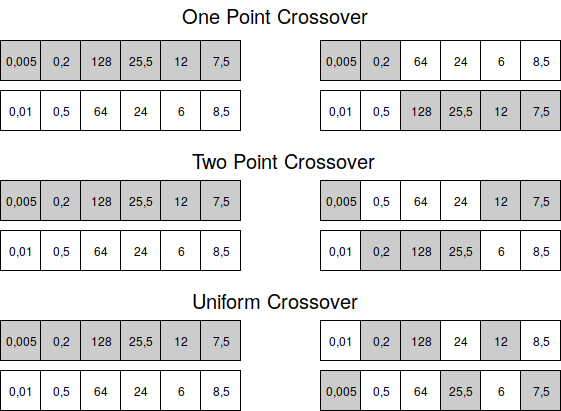
\includegraphics[scale=0.5]{img/crossover_gene.png}
  \caption{Die Wichtigsten drei Crossover Operationen. Oben die one-point Crossover, mitte two-point Crossover, unten Uniform Crossover. Auf der linken Seite sind Eltern abgebildet und auf der Rechtenseite die neu erzeugten Kinder}
  \label{fig:chromoson_crossover}
\end{figure}

Crossover nach dem Paper \cite{Umbarkar2015}.




\paragraph{Mutation} Hierbei wird jedes Gen des Individuums zufällig mit einer zufälligen Mutation versehen. Durch diese Mutation wird eine höhere Diversität in die nachfolgende Generation übergeben. Diese Mutation macht es möglich einen größeren Suchraum abzudecken und somit die Werte genauer anzupassen, um so auf die optimale Lösung zu kommen. Hier wird die Gauss-Mutation verwendet. Es wird ein Zufallswert aus der Normal- oder Gauß-verteilung hinzu addiert. Durch diese Wahrscheinlichkeitsverteilung werden viele Mutationen nur kleine Veränderungen, aber auch größere Sprünge sind möglich. Um die vorher mit Crossover neu bestimmten Individuen, welche schon eine hohe Grundfitness haben, nicht zu stark zu verändern wird ein Gen nur um wenige Prozent verändert. Dies ist in Abbildung \ref{fig:chromoson_mutation} zusehen. Die Mutationen in der Zeichnung wurden zufällig gewählt. 

Evolutionäre Algorithmen S.60


\begin{figure}[H]
  \centering  
  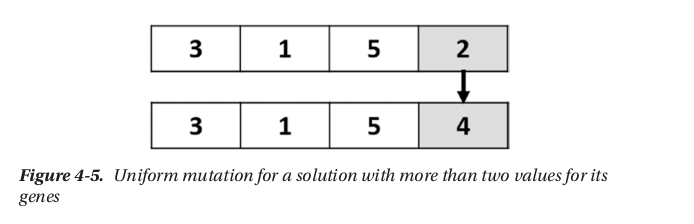
\includegraphics[scale=0.7]{img/mutation.png}
  \caption{Muation von Genen um eine höhere Diversität zu erhalten}
  \label{fig:chromoson_mutation}
\end{figure}

Practical Computer visionaplica ss.140
 
\subsubsection{Neue Generation}
Der letzte Schritt des Genetischen Algorithmuses besteht aus dem Austausch der Generationen. Die neue Kind Generation tauscht nun die alte Eltern Generation aus. Anschließend folgen die gleichen 4 Schritte so lange bis die gewünschte Fitnesswert erreicht ist. Nach dem erreichen der Abbruchbedingung, kann aus der letzten Generation das qualitativ hochwertigste Individuum ausgesucht werden und als Lösung verwendet werden.

\newpage

\subsection{Künstliche Neuronale Netze}

Künstliche Neuronale Netze sind dem natürlichen Vorbild der neuronalen Netze im Gehirn nachempfunden. Beide Netze setzen sich aus einzelnen Neuronen zusammen, welche miteinandern verbunden sind und somit ein großes Netz entstehen lassen. Wie man in Figure \ref{fig:neural_network} sieht ist jede Schicht aus einzelnen Neuronen aufgebaut, welche mit den Neuronen der nächsten Schicht verbunden sind. Diese Verbindungen repräsentieren die Gewichte, über diese kann einem Netz verschiedene Zusammenhänge von Input und Output antrainiert bzw. angelernt werden.



Im folgenden Kapitel wird zuerst der Aufbau eines Neurons/Perseptron erklärt. Anschließend wird auf den strukturellen Aufbau eines Künstlichen Neuronalen Netzes nähergebracht. Zum Schluss werden noch wichtige Eigenschaften wie die Verlustfunktion und der Gradientenabstieg eingegangen, sowie auf die Hyperparameter, welche für die Arbeit essenziell sind.



Grundlagen aus dem Buch ArificalNeuroalNetworks s.11 


\subsubsection{Aufbau eines Neurons}
\label{Aufbau eines Neurons}
Ein Neuron besteht immer aus dem gleichen Aufbau: Eingänge, Gewichte, Schwellwert, Aktivierungsfunktion und einem Ausgang.
Nachfolgenden Unterkapitel werden diese Ausführlich erklärt.
\begin{figure}[htb]
  \centering  
  \includegraphics[scale=0.9]{img/neuron.png}
  \caption{Aufbau eines Neurons}
  \label{fig:neuron}
\end{figure}


\paragraph{Eingang}
Bei den Eingangswerten $i_1, ..., i_n$ handelt es sich um einfache xxxFloatwertxxx, diese werden mit den Gewichten $w_1, ..., w_n$ verrechnet. Ein Neuron hat meist mehrere Eingangsgrößen, welche alle zusammen mit den Gewichten und dem Schwellwert aufsummiert werden. \ref{eq:4} Diese Werte werden zufällig initialisiert und per Training verbessert, somit handelt es sich um einen angelernten Werte, welche durch die Fehlerrückführung (engl. Backproagation) verbessert werden.

\paragraph{Schwellwert}
Auf dieses Aufsummiertes Ergebniss wird anschließend ein Schwellwert (engl. Bias) $w_0$ gerechnet, dieser führt zu einem besseren Verhalten beim Trainieren. Bei diesen Werten handelt es sich auch um angelernte Werte und helfen die Flexibitlität der Netze zu erhöhen.

\begin{equation}
	x = \sum_{k=1}^n i_k * w_k + w_0 \label{eq:4}
\end{equation}

\paragraph{Aktivierungsfunktion}
Die Aktivierungsfunktion kann man sich als Schwellwertfunktion vorstellen, ab wann das Neuron den Eingang weiter gibt.
Die entstandenen Summe x wird Aktivierung genannt und anschließend über eine Aktivierungsfunktion transformiert:
\begin{equation}
	o = f(x) \label{eq:5}
\end{equation}
Die Aktivierungsfunktion kann dabei verschiedene Formen haben. Für einfache Aufgaben kann Beispielsweise eine Sprungfunktion verwendet werden:
\begin{subnumcases}
{\sigma(t) = }
1, & wenn $t \geq 0$\\ \label{eq:6a}
0, & sonst $t < 0$		\label{eq:6b}
\end{subnumcases}

Für das approximieren von wertkontinuierlichen Funktionen wird die Sigmoid Funktion verwendet.
\begin{equation}
	sig(t) = \frac{1}{1 + e^{-t}} \label{eq:7}
\end{equation}
Bei der Klassifikation werden hingeben, der ReLU-Layer \ref{eq:8a} \ref{eq:8b} oder der Leaky-ReLU Layer \ref{eq:9a} benutzt, diese verhindern das Explodieren bzw. Verschwinden des Grandienten beim Training:
\begin{subnumcases} 
{R(z) = }
1, & wenn $z \geq 0$\\  \label{eq:8a}
0, & sonst $z < 0$		\label{eq:8b}
\end{subnumcases}
\begin{subnumcases} 
{R(z) = }					
1, & wenn $z \geq 0$\\		\label{eq:9a}
\alpha z, & sonst $z < 0$	\label{eq:9b}
\end{subnumcases}




\paragraph{Ausgang}
Wenn die Schwellwertfunktion aktiviert wird, wird am Ausgang des Neurons ein Wert geschalten. Dieser Ausgangswert kann dann entweder an andere Neuronen weitergeben werden oder als finales Ergebnis verwendet werden.


\subsubsection{Struktureller Aufbau eines Künstlichen Neuronalen Netzes}
Aus schlauem zusammen schließen solcher Neuronen entsteht ein Künstliches Neuronales Netz welches auch Multi-Layer-Perseptron genannt wird. Dabei sind grundsätzliche jegliche strukturelle Anordnung der Neuronen möglich. Besonders verbreitet ist das sogenannte Feedforward Netz (FFW).
Bei den FFW Netzen sind die Verbindungen nur in eine Richtung gerichtet. Dies wird beispielhaft in Abbildung \ref{fig:neural_network} gezeigt. Hier ist gut zu sehen, dass diese Netze in drei Schichten unterteilt werden können.  

\begin{figure}[htb]
  \centering  
  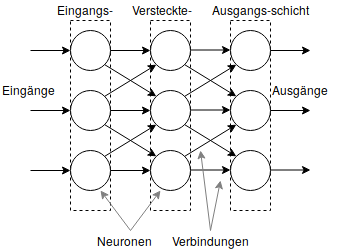
\includegraphics[scale=0.9]{img/mlp.png}
  \caption{Künstliches Neuronales Netz mit drei Schichten je drei Neuronen}
  \label{fig:neural_network}
\end{figure}


\begin{itemize}
\item \textbf{Eingangsschicht} Die Neuronen der Eingangsschicht sind nicht wie die in \ref{Aufbau eines Neurons} beschriebenen Neuronen aufgebaut. Die einzige Aufgabe der Eingangsneuronen ist das verteilen der Eingagsinformationen an die Versteckteschicht, weshalb es immer genau soviele Eingangsneuronen wie Eingangssignale geben muss.

\item \textbf{Versteckteschicht}
Die Verstecktesicht besteht aus den in \ref{Aufbau eines Neurons} erläuterten Neuronen. Sie kann aus einer Beliebigen Anzahl dieser aufgebaut sein. Es kann auch beliebig viele Versteckteschichten geben. In der Literatur bezeichnet man Neuronale Netze mit mehr als einer Verstecktenschicht als Deep Neural Networks.

\item \textbf{Ausgangsschicht}
Die Ausgangsschicht beinhaltet genau soviele Neuronen wie Ausgangsgrößen gewünscht.
Aus dieser können dann die Klassifizierungswerte entnommen werden.
\end{itemize}


\subsubsection{Verlustfunktion}
Die Verlustfunktion(engl. Lossfunction) stellt ein ausgesuchtes Maß der Diskrepanz zwischen den beobachteten und den vorhergesagten Daten dar. Sie bestimmt die Leistungsfähigkeit des Künstlichen Neuronalen Netzes während des Trainings. Ziel ist es, im laufenden Prozess der Modellanpassung, die Verlustfunktion zu minimieren.

\subsubsection{Gradientenabstieg}
Um die Fehlerfunktion zu minimieren wird als Werkzeug der Gradientenabstieg benutzt. Diese ist nur möglich, da ein Künstliches Neuronales Netz aus verketteten differenzierbaren Gewichte der Neuronen(Tensoroperationen) aufgebaut ist, die es erlauben duch Anwendung der Kettenregel die Gradientenfunktion zu finden, die den aktuellen Parametern des Datenstapels Werte des Gradienten zuordnet. Es gibt auch hier verschiedene Ansätze von Optimierern, welche die genauen Regeln wie der Gradient der Verlustfunktion zu Aktualisierung der Parameter verwendet wird hier könnte Beispielweise den RMSProp-Optimierer, der die trägheit des Gradientenabstiegsverfahren berücksichtet.

Seite 83 - Deep Learning chollet


\subsubsection{Hyperparameter}
Als Hyperparameter werden, in Bezug auf Künstliche Neuronale Netze, werdem meist die Anfangsbedingungen bezeichnet. 
Für diese Hyperparameter gelten keine universellen Werte sondern müssen je nach Daten und Funktion bzw. künstliches Neuroales Netz speziell angepasst und verändert werden. Deshalb gibt es nur einige Regeln und grobe Abschätzungen in welchen Grenzen sich diese Hyperparameter befinden. Zu diesen Hyperparameter gehören folgdende:
\begin{itemize}
\item \textbf{Learningrate},blabalaa
\item \textbf{Dropout}
\item \textbf{Lossfunktion}
\item \textbf{Optimizer}
\item \textbf{Model Achitektur}
\end{itemize}

xxxwird noch angepasst wenn ich weis welche Parameterxxx

\subsection{Zusammenfassung}


\iffalse
Genetische algorithms ist ein sehr erfolgreiches Oprimiungsverfahren welches es erlaubt auch bei schweren Suchräumen lösungen zu finden. Insbesondere wenn keine gradienten berechnet werden können. In diesem Kapitel wurden die Grundlagen der genetischen Grundlagen zusammengefasst. Sie bassieren auf einer Lösungspopulation, die sich im laufe der iterationen dem Optima annähert. Genetische Operatioren ändern die Lösungen. Cross-overoperatoren kobinieren genome zweier Lösungen. Die Mutation fügt den Lösungen Zufälligkeiten hinzu und sollte somit jenden Ort im Lösungsraum erreichen. Der Genotyp oder Das Chromosom einer Lösing wird auf einen Phänotyp, die reale Lösung, abgebildetet, bevor es mit einer Fintessfunktion ausgewertet werden kann. Diese Fittnesfunktion muss sehr sorgfällig ausgearbeitet werden, da sie einen entscheidenden einfluss auf die Suche hat. Die Lösungen mit der höchsten fittnes sind folglich die Eltern der nächsten generation. Sobald eine Generation eine bestimmte Fintess ereicht sprich genug Optimiert wurde ist die beste Lösung gefunden. Somit wurde ein Algorithmus vorgestellt welcher auf ein breites Spektrum von Probkemen anwendbar ist.

Genectic - algorhmen - essential s.19 
\fi
